\documentclass[oneside, twocolumn, a4paper, 10pt]{IEEEtran}
\usepackage{caption}
\usepackage{url}
\usepackage[dvipsnames]{xcolor}
\usepackage{graphicx}
\usepackage{hyperref}
\usepackage{program}
\begin{document}
\title{Interpretable Clustering and Classification of an Imbalanced Dataset of DNA Sequences}
\author{Shekh Ahammed Adnan Bashir \\ Department of Computer Science and Engineering \\ Bangladesh University of Engineering and Technology \\ \url{1018052026@grad.cse.buet.ac.bd}}
\date{\today}
\maketitle

\begin{abstract}
Clustering or classification of DNA sequences is more difficult than doing those with any other type of sequences due to various reasons. Such tasks become more difficult when they have to be done on genus or family. Further difficulty is added when the class samples vary in number- that is, the dataset of DNA sequences is imbalanced. However, through using proper feature extraction techniques and dataset sampling technique such tasks are becomes feasible. The dataset we work with in this paper has $9$ classes and the number of samples vary from $4$ to $1269$. In this work, we present a feature extraction technique inspired by popular Natural Language Preprocessing algorithm GloVe \cite{1} to make the classification and clustering of such huge and imbalanced dataset possible. The feature extraction routine is static rather than being a learning one. This eased the interpretation of the machine learning tasks easier. Using interpretable shallow learning techniques, we achieved an accuracy score around $99.8$\% and a V-measure of $0.5363$.
\end{abstract}

\section{Introduction}
As the rapid development of next generation genome sequencing techniques, newer species are being classified quickly. It is important to know the class (family or genus) that a newly sequenced DNA belong to besides learning how the new species are related to the other ones. Here comes the necessity of DNA sequence classification and clustering. In both classification and clustering, a given collection of items is separated into a few to several subcollections so that the items in one subcollection are as similar as possible with items in two different subcollections are as different as possible. However, they differ in the way they do it.\\
\par
In classification, labeled data is provided to the classifier and the classifier learns an implicit measure of similarity upon seeing the labels of the provided data. This implicitly learned similarity measure can take a very compilcated mathematical form. On the other hand, in clustering a measure of similarity is provided explicitly and the clusterer sperataes the items into subcollections according to that similarity score. The clusterer does not need data labels. The better the similarity measure provided to the clusterer, the better the separation is and hence better the V-measure score is. As the similarity measure used in clustering is already understood, we can gain an insight into the data in the light of that. Broadly speaking, classification discovers the spearating boundary in a given collection to divide that into subcollections and clustering is discovering the groups based on a provided similarity measure. Clustering provides us a view of how the items in a collection form homogeneous groups of items and classification draws decision boundaries among the groups.\\
\par 
A sequence is a list of elements. In a sequence, items of the provided collection are arranged one after another. There might or might not be sequential dependencies among the items. That is, value of an item appearing in the latter positions might or might not depend the value of item or items appearing in the previous positions. This dependency relation varies from problem to problem and this can only either be inferred from the data or provided to the algorithm as parameters. Classification and clustering tasks on the sequences hence are very difficult with data analysis and static algorithms only.\\
\par
DNA sequences are composed of $4$ different nucleotides- Adenine, Cytosine, Guanine, and Thiamine. Therefore, it is very likely that DNA sequence of two species share some common region because of the small state space. There are noises in the DNA sequences. There are intra-class difference of the DNA sequences when it comes classifying genus or families of DNA sequences. Through using preprocessing techniques that maintains the class invariant properties yet transforming all the sequences into sequences of same length or extracting features we can successfully classify or cluster the sequences in such cases.\\
\par
Interpretability is important to better understand the data so that some static algorithm can be employed to do something of importance with a certain guarantee. When a classifier or a clusterer does their repective tasks, it can do so interpretably or not. Using static feature preprocessing and understanding the parameters and attributes of the machine learning models helps result interpretation. Decision tree based classifiers, probabilistic classifiers, manifold learning algorithms provide interpretable results because they do their in a predefined step by step manner rather optimizing the decision boundary based on different hyperparameters only like black box machine learning models.\\
\par
In this work, our main focus has been on interpreting the results obtained from the clusterer and the classifier. Specifically, our contributions are:
\begin{itemize}
\item Designing a feature extraction procedure that maintains the class invariant property of the DNA sequences.
\item Using interpretable machine learning techniques to cluster and classify the DNA sequences.
\item Interpretation of the results obtained from the clusterer and the classifier.
\end{itemize}

%
\section{Previous Works}
Better the features better the classification accuracy is. Works done so far on the classification of DNA sequences first extracts features. Nearly all the feature extraction procedure are hand engineered features. Also many of them do not employ popular classification algorithms on those hand-engineered extracted features. Many of them incorporates the use of very popular DNA sequence matching algorithm BLAST for thr discrimination of the sequences purpose. Wang et al. proposed two new methods to classify DNA sequences \cite{2}. The first technique relies on the comparison of a given sequence to a group of active motifs discovered from the classes it knows. The second technique generates and matches gapped fingerprints of a given unlabeled sequence with the elements of classes it knows. Stranneheim et al. classified DNA sequences through using Bloom filters to keep track of novelties of the sequence reads \cite{3}. Seo transformed sequence data to real-valued vectors so that Support Vector Machine (SVM) can be applied \cite{4} to the data for the purpose of classification. In MEGAN \cite{5}, a sequence is searched against multiple sequence databases for assigning the lowest common ancestor of the best matches in different databases to the sequence. PhymmBL \cite{6}, \cite{7} uses interpolated Markov models to characterize variable-length oligonucleotides and combines with BLAST matching score to yield better accuracy. The Na\"{i}ve Bayes classifier \cite{8} learns a Bayesian rule from the k-mer distribution of genomes in the training data and applies that rule to classify. In Kraken \cite{9}, each k-mer in the sequence is mapped to the lowest common ancestor (LCA) of the genomes that contain that k-mer in a database. For classifcation, the taxa associated with the k-mers in the sequence form a pruned subtree of the general taxonomy tree. Another classifier CLARK \cite{10} defines k-spectrum. k-spectrum of a string $x$ is the vector of dimension $4^k$ that collects the number of occurences of all possible k-mers in $x$. k-spectrum represents each DNA sequence. The CLARK algorithm first computes the k-spectrum of a unlabeled DNA sequence. Then the algorithm removes the common regions of the sequences to make the remaining k-mers to be discriminative. Finally, based on the maximum similarity in k-mer frequencies a class is assigned to an unlabeled DNA sequence.\\
\par
As we already discussed, clustering of DNA sequences is done to study the similarities among the DNA sequences through the lens of a predefined similarity measure. Plenty of works, such as DNACLUST \cite{11}, d2 cluster \cite{12}, CD-HIT \cite{13}, UCLUST \cite{14} have already been done to cluster DNA sequences and they are interpretable. However, seldom of them used adhoc clustering algorithms rather than the ones which are widely known and their inner workings are understood in depth. MeShClust \cite{15} addressed the issue of the sensitivity of clusterer output due to predefined algorithm paramaters. It repurposes the popular Mean Shift algorithm \cite{16} for the DNA sequence clustering. It is a nonparametric feature space analysis technique and seeks the maxima of a density function. The space spanned by DNA sequences can be considered as feature space. The distribution has a density function in that space and modes are the cluster in the input space. However, considering the maxima of the density function as in Mean Shift algorithm makes it very difficult to work with highly imbalanced training dataset- that is, if the number of samples from different classes varies largely.
\section{Methodology}
\subsection{Sequence Embedding}
\subsubsection{Popular techniques}
Embedding is the process of mapping some signal from one domain to another. It is done for the convenience of postprocessing. Sequence embedding maps an entire sequence to another domain. Sequence embedding eases the modeling the sequence for further tasks. Sequence modeling is predicting the distribution of the smaller units of the sequence. It also can be used to extract features of the sequences. Feature extraction falls under the umbrella of feature learning. Feature extraction is done through discovering the patterns among the smaller units in the sequence. Feature extraction routines can be learning procedures or static procedures. Therefore, feature extraction can be done using static algorithms those rely on domain specific knowledge or hypotheses regarding the sequence or can be done using neural networks or shallow learning algorithms.\\
\par 
In the field of Natural Language Processing, word embedding, which is a sequence embedding technique, refers to a set of techniques for language modeling and feature learning. In NLP, word embedding is done on words or phrases to map them to real valued vectors. This real-valued vectors are used for further tasks- such as classification or clustering. There are severalp opular word embedding techniques including word2vec \cite{17}, GloVe \cite{18}, fastText \cite{19} \cite{20}, etc. Each of the routines transforms word sequences such as sentences, paragraphs, etc. into real valued vectors for feasible classification, clustering, etc.\\
\par 
word2vec reduces the number of dimensions using neural networks to learn the embedding. It produces the sequence embedding in two exclusive methods. In one method, called continuous bag of words, the feature learning model is trained to predict a word from the context or surrounding words of it. In another method, called skip-gram, the context words are predicted from a given word through assigning some probability score to a one hot vector of the vocabulary under consideration. GloVe uses a static method to produce the embedding. GloVe model is trained on aggregated global word-word co-occurrence statistics from a corpus. Representations obtained from GloVe demonstrate interesting linear substructures of the word vector space. fastText learns a representation for each character n-gram (a number of neighboring characters around a character in a word) instead of directly learning a vector representation for a word (as with word2vec). Each word is represented as a bag of character n-grams, so the overall word embedding is a sum of these character n-grams.
\subsubsection{Our approach}
We extend two sequence embedding techniques to the domain of biological sequences- word2vec and GloVe. However, rather directly using them, we modify them for using with k-mers. As k-mers we pick 3-mers, that is the codons. We did not pick the value of $k$ experimentally. We picked a value of $k$ that corresponds to a already known and studied biological structure.\\
\par
We first split the sequence into nonoverlapping subsequence of length $k$. Then we construct a \textit{weighted} cooccurence vector out of that. To construct the vector we first define a number of neighbors on the right and the left side of a given k-mer and initialize and a matrix of $0$s of dimension $4^k \times 4^k$ with $4$ being the number of DNA bases and $k$ being the $k$ value of the k-mer we consider. Therefore, the rows and the columns of the matrix corresponds all possible k-mers. That is, an item $C_{i,j}$ is the weight of association between k-mer $i$ and k-mer $j$ in a given sequence. We call this matrix cooccurence matrix.\\
\par
We take maximum that number of left and right neighbor. For example, for a sequence of length $100 * k$ (k-mer sequence of length $100$) and left and right neighbor count of $3$, the first k-mer in the sequence we only have the right neighbor (k-mers in the $2^{nd}$, $3^{rd}$, and $4^{th}$ positions), the last k-mer has only left neighbors (k-mers in the $97^{th}$, $98^{th}$, and $99^{th}$ positions), and the $10^{th}$ k-mer has k-mers in $7^{th}$, $8^{th}$, and $9^{th}$ position as the left neighbors and k-mers in the $11^{th}$, $12^{th}$, and $13^{th}$ positions in the sequence as the right neighbors. Now we add $\frac{1}{3}$ to the weight between the k-mer at the $10^{th}$ position and the k-mer at the $7^{th}$ position and the k-mer at the $10^{th}$ position and the k-mer at the $13^{th}$ position. That is, we do $\mathbf{C}_{10, 7} = \mathbf{C}_{10, 7} + \frac{1}{3}$ and $\mathbf{C}_{10, 13} = \mathbf{C}_{10, 13} + \frac{1}{3}$. We also do $\mathbf{C}_{10, 8} = \mathbf{C}_{10, 8} + \frac{2}{3}$ and $\mathbf{C}_{10, 12} = \mathbf{C}_{10, 12} + \frac{2}{3}$ and finally, $\mathbf{C}_{10, 9} = \mathbf{C}_{10, 9} + 1$ and $\mathbf{C}_{10, 11} = \mathbf{C}_{10, 11} + 1$. Finally, we flatten the matrix to obtain the cooccurence vector, that is, $\vec{C} = \mathbf{C}_{1,1}, \ldots, \mathbf{C}_{1, N}, \mathbf{C}_{2, 1}, \ldots, \mathbf{C}_{2, N}, \ldots, \mathbf{C}_{N-1, N},\mathbf{C}_{N, 1}, \ldots, \mathbf{C}_{N, N}$. Later, we divide the vector with the largest element in it in order to normalize it. This is how we get feature vector of constant size. The significance of this vector can be thoght of to express cooccurence intensity between the k-mers.
\subsection{Visualization through dimension reduction algorithms}
Many datasets can be represented as a matrix, such that each row represents a set of attributes (or features or dimensions). Attributes describe a particular instance of something. Larger the number of attributes (columns) exponentially large the space of unique possible rows. Large number of data dimension causes difficulties in data sampling and pattern recognition. Reducing data into fewer dimensions often makes the analysis of algorithms more efficient, and can help machine learning algorithms make more accurate predictions.\\
\par
We want to have our clusters as nonoverlapping as possible. Visualization is important to understand how good our embedding routine is. We first visualize the clusters through dimension reduction algorithms. We pick three algorithms for that:
\begin{itemize}
\item Isomap
\item Locally-Linear Embedding (LLE)
\item T-distributed Stochastic Neighbor Embedding (t-SNE)
\end{itemize}
\begin{figure*}
\centering
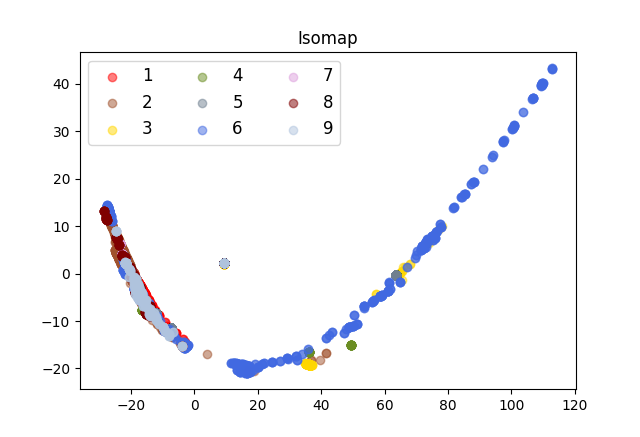
\includegraphics[width=0.6\linewidth]{../data/visualization/Isomap.png}
\caption{Isomap on the embeddings obtained from our embedding algorithm.}
\label{fig:isomap}
\end{figure*}
In Isomap first neighbors of each data point are found. Then a neighborhood graph is constructed with each point is connected to other if it is a $K$ nearest neighbor and edge length equal to Euclidean distance. Then in that neighborhood graph the shortest path between the nodes are computed. Finally, a lower-dimensional embedding is computed using multidimensional scaling. We notice that in the Isomap plot \autoref{fig:isomap} of our features many classes are largely overlapped.\\
\par
\begin{figure*}
\centering
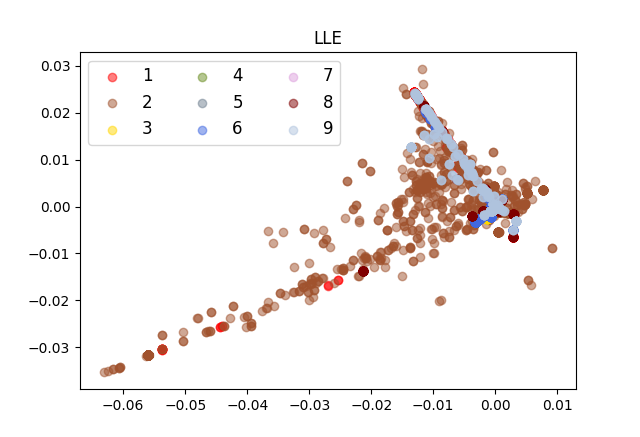
\includegraphics[width=0.6\linewidth]{../data/visualization/LLE.png}
\caption{Locally-Linear Enbedding on the embeddings obtained from our embedding algorithm.}
\label{fig:lle}
\end{figure*}
Locally-Linear Enbedding leverages the sparsity of the data matrix. First, LLE finds a set of the nearest neighbors of each point. Then it computes a set of weights for each point that best describes the point as a linear combination of its neighbors. Finally, an eigenvector-based optimization is done to find the low-dimensional embedding of points, such that each point is still described with the same linear combination of its neighbors. LLE does not have a mechanism to work with data points with nonuniform density. It performs poor in those cases. This is observed in our LLE plot \autoref{fig:lle}.\\
\par
\begin{figure*}
\centering
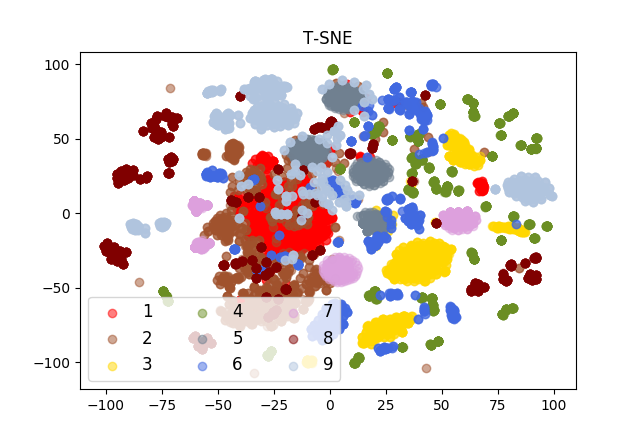
\includegraphics[width=0.6\linewidth]{../data/visualization/T-SNE.png}
\caption{T-distributed Stochastic Neighbor Embedding on the embeddings obtained from our embedding algorithm.}
\label{fig:tsne}
\end{figure*}
t-SNE models each high-dimensional data point by a two- or three-dimensional point in such a way that similar objects are modeled by nearby points and dissimilar objects are modeled by distant points with high probability. First, a probability distribution over pairs of high-dimensional objects is constructed. Second, a similar probability distribution is defined over the points in the low-dimensional map, and then t-SNE minimizes the Kullback–Leibler divergence between the two distributions with respect to the locations of the points in the map. Reducing dimensionality with t-SNE we are able to see the clusters better upon plotting \autoref{fig:tsne}. However, feeding this reduced dimensioned data to the classifiers does not yield better classification.\\
\par
This is error is due to the unsupervised nature of the dimension reduction algorithms. The classification boundary in all problems cannot be properly defined by the well-studied similarity measure(s) alone. Therefore, dimension reduction in an unsupervised fashion does not always work. This is the reason we did not reduce the data dimension for supervised training.
\subsection{Sequence Clustering}

\subsection{Sequence Classification}
\section{Interpretation}
%
%\section{Methodology}
%\subsection{Suitability of Machine Learning Model in this Setting}
%One starting point to detect filtered images can be noticing the color distribution. This is because we are interested in exploiting color information to detect filtered images. A color histogram is the representation of the count of pixels with a specific color. For an RGB image, the color histogram consists of the number of red pixels with different values of intensity, the number of green pixels with different values of intensity, and the number of blue pixels with different values of intensity. We remember that image filters modify the image pixels in a certain manner to produce filter effects. However, as in \autoref{fig:filter-hist-bird} and \autoref{fig:filter-hist-sun} color distribution is not of that much help. Color distribution of a given filter varies over the content.
%\begin{figure*}
%\centering
%\includegraphics[width=0.75\linewidth]{bird-natural.jpg}
%\centering
%\includegraphics[width=0.75\linewidth]{bird-gotham.jpg}
%\centering
%\includegraphics[width=0.75\linewidth]{bird-kelvin.jpg}
%\centering
%\includegraphics[width=0.75\linewidth]{bird-lomo.jpg}
%\centering
%\includegraphics[width=0.75\linewidth]{bird-nashville.jpg}
%\centering
%\includegraphics[width=0.75\linewidth]{bird-sepia.jpg}
%\centering
%\includegraphics[width=0.75\linewidth]{bird-toaster.jpg}
%\centering
%\caption{From top to bottom: A digital RGB image of a bird (randomly taken from the OpenImages v4 dataset \cite{14}) and its color histogram, Gotham filtered image of the same image and its color histogram, Kelvin filtered image of the same image and its color histogram, Lomo filtered image of the same image and its color histogram, Nashville filtered image of the same image and its color histogram, Sepia filtered image of the same image and its color histogram, and Toaster filtered image of the same image and its color histogram.}
%\label{fig:filter-hist-bird}
%\end{figure*}
%\begin{figure*}
%\centering
%\includegraphics[width=0.75\linewidth]{sun-natural.jpg}
%\centering
%\includegraphics[width=0.75\linewidth]{sun-gotham.jpg}
%\centering
%\includegraphics[width=0.75\linewidth]{sun-kelvin.jpg}
%\centering
%\includegraphics[width=0.75\linewidth]{sun-lomo.jpg}
%\centering
%\includegraphics[width=0.75\linewidth]{sun-nashville.jpg}
%\centering
%\includegraphics[width=0.75\linewidth]{sun-sepia.jpg}
%\centering
%\includegraphics[width=0.75\linewidth]{sun-toaster.jpg}
%\centering
%\caption{From top to bottom: A digital RGB image of the Sunderbans \cite{17} and its color histogram, Gotham filtered image of the same image and its color histogram, Kelvin filtered image of the same image and its color histogram, Lomo filtered image of the same image and its color histogram, Nashville filtered image of the same image and its color histogram, Sepia filtered image of the same image and its color histogram, and Toaster filtered image of the same image and its color histogram.}
%\label{fig:filter-hist-sun}
%\end{figure*}
%If we have a computational model to capture the color information of images, we can build a classifier to recognize filtered images. This computational model can be anything from an exact algorithm to a machine learning model. An exact algorithm is very difficult to build to serve this purpose because of an extremely large number of different cases to be handled. For instance, a naive approach could have been thresholding the peaks of the color histograms. However, this might fail, because various factors affect the color histogram. These factors include- occlusion of objects in an image, the angle of the image, illumination condition, image quality in terms of noises due to the camera, etc. Machine learning models can conveniently learn these cases implicitly. However, shallow machine learning models need a lot of tuning and a lot of hand-written cases. Also, several machine learning models have to be employed to learn different features and later outputs of those models are to be ensembled to build the final model.\\
%\par
%A computational model is essentially a function computing an output given some inputs and parameters. Deep neural networks can solve any problem if those are trained to capture, that is- learn, a specific function through backpropagation for many epochs. A deep neural network model can be trained end-to-end in a supervised manner to solve any problem \cite{11}. Therefore, through using a proper dataset and a proper neural network architecture, we can build a classifier to recognize filtered images.
%\subsection{Neural Networks to Recognize Filtered Images} 
%The neural network architecture is the way neurons are arranged in a neural network. Convolutional neural networks are best suited for tasks involving images or videos as first shown by the Krizshevsky et al \cite{12} and later being proven again and again as evidenced in the literature of computer vision. In \cite{13}, the authors showed that residual networks learn to classify images with better accuracy than the other existing convolutional neural network architectures. This is because residual networks produce a better representation of images than other ones. Also, the depth of a residual network can be made arbitrarily large so that better representation can be learned from the output of the previous layer in the neural network.\\
%\par  
%Detection of unseen filtered images (images filtered with image filters unseen at the training time of the model) is important because there can be endless image filters designed. Also, we need to be able to recognize resultant images of as many unknown image filters as possible. In this work, I have trained a deep neural network that leverages deep representations from two different neural networks to recognize filtered images. Further, I also trained a deep neural network that leverages representations from three neural networks. I showed that by training a tri-modular classifier on samples of only 2(3) image filters, we can recognize results of 6 image filters despite noticeable difference in the final output of the filters.\\ 
%\par
%End-to-end trained neural network model on different image filters have a large number of parameters and hence take a lot of time to evaluate an image. Larger the number of image filters such a neural networks sees during training, the number of parameters gets larger. We have found that through taking a bi-modular(tri-modular) approach in designing neural network architecture. Each module is a classifier trained to recognize one single image filter and finally these networks are used to extract deep representations those are in turn used to train a neural network to detect filtered images. This neural network acts as a voter in an N-modular system and trained on the dataset of natural images and their filtered counterparts. Only 2(3) image filters are used at this point to generate the training dataset. Rest among 6 filters are used to generate the testing dataset. Now we present the steps we followed during the work. \autoref{tab:comparison2} and \autoref{tab:comparison3} shows the accuracy of the models we trained in this paper.
%\\
%\par
%We resized the images in the dataset to $64 \times 64$ pixels so that colors are globally considered by the classifier while ignoring image objects as much as they can. Then two neural networks with the same architecture are trained to distinguish natural images and their Nashville/Toaster filtered counterparts. Another classifier \autoref{fig:weak-sepia} with a different architecture and smaller number of parameters is trained to distinguish natural images and their Sepia filtered counterparts. Our experiments showed that with a smaller number of parameters such a classifier can be constructed.
%\begin{figure*}
%\centering
%\includegraphics[width=0.25\linewidth]{Weak-sepia.png}
%\centering
%\caption{Natural vs Sepia filtered image classifier.}
%\label{fig:weak-sepia}
%\end{figure*}
%\begin{figure*}
%\centering
%\includegraphics[width=0.2\linewidth]{extractor.png}
%\centering
%\caption{Part of the binary classifier trained to detect Natural versus Nashville/Toaster filtered images. For brevity, we are showing only the layers that contribute to the feature we extract.}
%\label{fig:extractor}
%\end{figure*}
%Features with dimension (8, 8, 32) are extracted from the classifier \autoref{fig:extractor} of Nashville and Toaster and features with dimension (8, 8, 16) are extracted from the leaky\_re\_lu\_5 layer of the classifier \autoref{fig:weak-sepia} of Sepia filtered images. These features are stacked as suitable for bi-modular/tri-modular approach and used as input to another neural network that works similar to a voter. Now we look at the architecture of one of the sequential network we trained as voter \autoref{figure:voter}. This is the best performing Bi-Modular classifier we have constructed. 
%\begin{figure*}
%\centering
%\includegraphics[width=0.35\linewidth]{Ensemble-small.png}
%\centering
%\caption{Voter Neural Network Architecture of Bi-Modular-Large.}
%\label{figure:voter}
%\end{figure*} 
%\section{Experimental Evaluation}
%Over the course of the whole experiment, we have trained a lot of Neural Network based classifier. Only the best ones are presented here and used to produce results.
%\subsection{Dataset Compilation}
%InnerEye is aimed towards pictures available on Social Media. People can publish anything to everything on social media nowadays. Therefore, we picked a dataset that contains images of a very wide variety. We randomly subsampled $30,000$ images from the popular OpenImagesv4 dataset \cite{14}. This dataset includes samples of $19,794$ different classes. Then we applied Gotham, Kelvin, Lomo, Nashville, Sepia, and Toaster filters on the images \cite{15}.
%\subsection{Modules}
%The goal is to keep the number of filters seen at the training time small while increasing the number of filters we recognize at the deployment. We first trained weak binary classifiers to recognize natural images versus images filtered by one specific filter. In the table \autoref{tab:comparsion1} we see the performance of these binary classifiers on images filtered with different filters. We note that the classifier trained on Natural vs Nashville filtered images perform better than the rest of the classifiers on Kelvin filtered image but Kelvin binary classifier. Again, classifiers trained on Natural vs Toaster filtered images perform better than the rest of the classifiers on Gotham and Lomo filtered images but respectively Gotham binary classifier and Lomo binary classifier. Also, filters trained on Natural vs Gotham filtered images perform better than the rest of the classifiers on Nashville and Toaster filtered images but Nashville binary classifier and Toaster binary classifier. However, by choosing Nashville and Toaster binary classifier to be to extract features we have detection accuracy more than $60\%$ for all but Sepia filtered images.
%\begin{table*}
%\begin{center}
%%\begin{tabularx}{\columnwidth}{|l|X|X|X|X|X|X|}
%\begin{tabular}{|c|c|c|c|c|c|c|}
%\hline
%- & Gotham & Kelvin & Lomo & Nashville & Sepia & Toaster \\ \hline
%Gotham & \textcolor{ForestGreen}{96.27} & 49.9 & 53.35 & 60.91 & 49.84 & \textcolor{RoyalBlue}{67.61} \\ \hline
%Kelvin & 49.08 & \textcolor{ForestGreen}{99.88} & 49.62 & \textcolor{RoyalBlue}{65.4} & 49.84 & 50.35 \\ \hline
%Lomo & 88.74 & 50.02 & \textcolor{ForestGreen}{99.45} & 77.05 & 49.85 & \textcolor{RoyalBlue}{92.65} \\ \hline
%Nashville & \textcolor{RoyalBlue}{54.02} & 50.6 & 52.04 & \textcolor{ForestGreen}{83.28} & 49.91 & 52.8 \\ \hline
%Sepia & 47.66 & \textcolor{RoyalBlue}{49.92} & 49.63 & 47.11 & \textcolor{ForestGreen}{99.79} & 47.82 \\ \hline
%Toaster & \textcolor{RoyalBlue}{55.53} & 49.95 & 51.46 & 48.5 & 49.91 & \textcolor{ForestGreen}{94.65} \\ \hline
%\end{tabular}
%\end{center}
%\caption{Comparison of the weak binary classifier models on seen and unseen filters. Along the row is the binary model trained and along the column are the filters. Not one classifier does the best to detect images filtered by a given image filter. Greens are the best performant in the row. Blues are the second best performant in the row.}
%\label{tab:comparsion1}
%\end{table*}
%\subsection{Bi-Modular over End-to-End Appraoch}
%We have trained an End-to-End residual network on Nashville and Toaster filtered images along with natural images in order to compare the performance of Bi-modular approach over the End-to-End approach. We evaluated the accuracy of this classifier on all 6 filtered images as well as natural images. For each filter, our Bi-Modular classifier, BM-Large, performed better than the End-to-End classifier \autoref{tab:comparison4}. The End-to-End trained classifier has $168,130$ parameters. This is larger in parameters ($1.3537$ times larger) in comparison to the Bi-modular classifier with $124,202$ parameters. However, the accuracy of the End-to-End one is $73.42$ and that for the bi-modular one is $74.45$. That is, the accuracy of the bi-modular classifier is $1.0139$ times of that of the End-to-End trained one. For the rest part of this section, we try to perform better than this in terms of both accuracy and the number of parameters of the neural network.\\
%\par
%We have trained another Bi-modular classifier other than the one we discussed in the previous section to check if we can do better through leveraging deeper representation from weak binary classifiers. The previous one extracts features of dimension $8 \times 8 \times 64$ and this one- let's call that Bi-modular-Small, extracts features of dimension $4 \times 4 \times 256$. We note that, in terms of the number of elements of tensors, both the features are equal. The voter in the Bi-modular-Small has only one Dense layer. The architecture is given in \autoref{fig:voter-small}. The number of parameters is only $239,234$ and the accuracy is $75.22$. The End-to-End classifier has $0.7028$ times parameters than Bi-modular-Small and yet performs $0.976$ times better than Bi-modular-Small. Now we ask ourselves if we could do better with a deeper neural network instead of only one dense layer in the voter neural network.
%\begin{figure*}
%\centering
%\includegraphics[width=0.3\linewidth]{Ensemble-smaller.png}
%\centering
%\caption{Voter Neural Network Architecture of Bi-Modular-Small.}
%\label{fig:voter-small}
%\end{figure*} 
%\par
%We train two neural networks. One is sequential and another is residual. We call the first to be Bi-modular-Seq \autoref{fig:voter-seq} and the latter Bi-modular-Res \autoref{fig:voter-res}. Bi-modular-Seq has $387,074$ parameters which are $2.3$ times larger than the End-to-End classifier and the accuracy is $73.53$ which is only $1.002$ times better than that of the End-to-End classifier. Bi-modular-Res has $322,850$ parameters and has an accuracy of $74.51$ making it inferior to the End-to-End classifier by $1.9202$ times in the number of parameters and superior to the latter in accuracy by $1.0149$ times. %Bi-modular-Res   
%\begin{figure*}
%\centering
%\includegraphics[width=0.25\linewidth]{bm-seq.png}
%\centering
%\caption{Voter Neural Network for Bi-Modular-Sequential Classifier.}
%\label{fig:voter-seq}
%\end{figure*}
%\begin{figure*}
%\centering
%\includegraphics[width=0.2\linewidth]{bm-res.png}
%\centering
%\caption{Voter Neural Network for Bi-Modular-Residual Classifier.}
%\label{fig:voter-res}
%\end{figure*}
%\begin{table*}
%\begin{center}
%\begin{tabular}{|c|c|c|c|c|c|}
%\hline
%Filter & End-to-End & BM-Large & BM-Small & BM-Seq & BM-Res \\ \hline
%Gotham & 68.39 & \textcolor{RoyalBlue}{68.56} & \textcolor{OliveGreen}{70.53} & 67.67 & 67.89\\ \hline
%Kelvin & 84.28 & \textcolor{RoyalBlue}{85.8} & \textcolor{OliveGreen}{86.07} & 78.6 & 81.81\\ \hline
%Lomo & 81.51 & 82.36 & \textcolor{OliveGreen}{85.16} & 82.9 & \textcolor{RoyalBlue}{84.27}\\ \hline
%Nashville & 78.24 & 79.33 & 80.6 & \textcolor{RoyalBlue}{81.31} & \textcolor{OliveGreen}{81.58} \\ \hline
%Sepia & \textcolor{OliveGreen}{46.04} & \textcolor{RoyalBlue}{45.99} & 44.62 & 45.06 & 45.87 \\ \hline
%Toaster & 82.05 & 84.63 & 84.35 & \textcolor{RoyalBlue}{85.46} & \textcolor{OliveGreen}{85.65}\\ \hline
%%Parameters & \textcolor{RoyalBlue}{$168,130$} & \textcolor{OliveGreen}{$124,202$} & $239,234$ & $387,074$ & $322,850$\\ \hline
%%Agg. Acc. & $440.51$ & $446.67$ & \textcolor{OliveGreen}{$451.33$} & $441.0$ & \textcolor{RoyalBlue}{$447.07$}\\ \hline
%%Avg. Acc. & $73.42$ & $74.45$ & \textcolor{OliveGreen}{$75.22$} & $73.5$ & \textcolor{RoyalBlue}{$74.51$}\\ \hline
%%Param. per Acc. & \textcolor{RoyalBlue}{$2289.98$} & \textcolor{OliveGreen}{$1668.26$} & $3180.39$ & $5266.31$ & $4332.98$\\ \hline
%\end{tabular}
%\caption{Accuracy comparison of End-to-End trained and different Bi-modular classifiers to recognize filtered images. Accuracies are provided in percentage. Greens are the best performant in the row. Blues are the second best performant in the row.}
%\label{tab:comparison2}
%\end{center}
%\end{table*}
%\begin{table}
%\begin{center}
%\begin{tabular}{|c|c|c|}
%\hline
%Architecture & Number of Parameters & Accuracy\\ \hline
%End-to-End & \textcolor{RoyalBlue}{$168,130$} & $73.42$\\ \hline
%BM-Large & \textcolor{OliveGreen}{$124,202$} & $74.45$\\ \hline
%BM-Small & $239,234$ & \textcolor{OliveGreen}{$75.22$}\\ \hline
%BM-Seq & $387,074$ & $73.5$\\ \hline
%BM-Res & $322,850$ & \textcolor{RoyalBlue}{$74.51$}\\ \hline
%\end{tabular}
%\caption{Comparison of architectures we built models on. Greens are the best performant. Blues are the second best performant.}
%\label{tab:comparison4}
%\end{center}
%\end{table}
%\subsection{Tri-modular over Bi-modular Approach}
%We notice that both the End-to-End trained and Bi-modular classifiers are doing bad with Sepia filtered images. Therefore, picking up only the Nashville and Toaster filtered images to train is not enough. This is because the Sepia filter is based on convolution unlike the rest of the filters. Therefore, we build another dataset in the exact same process we did but include Sepia filtered images this time. Also, we build another weak classifier based on neural network \autoref{fig:weak-sepia} with a smaller number of parameters trained to distinguish between natural and Sepia filtered images. Final $11$ layers are removed from this neural network and use this as a feature extractor. We build a tri-modular in the same method we built the bi-modular classifier except we add one more module that is feature-extractor.
%\begin{figure*}
%\centering
%\includegraphics[width=0.35\linewidth]{tm.png}
%\centering
%\caption{Voter neural network for the Tri-Modular classifier.}
%\label{fig:tm}
%\end{figure*}
%This tri-modular classifier \autoref{fig:tm} has $129,586$ parameters and yields an accuracy of $80.47$ while the End-to-End trained classifier has $168,130$ parameters ($1.2974$ times parameters than the tri-modular classifier) and yields an accuracy of $82.69$ ($1.0221$ times accuracy). It is worth mentioning that this End-to-End classifier has the same architecture as the one we used before despite different training dataset. Bi-modular-Large yielded the best accuracy. Therefore, we compare the End-to-End classifier trained on Natural vs \{Nashville, Sepia, Toaster\} dataset, Bi-modular-Large, and the Tri-modular classifier we just trained \autoref{tab:comparison5}.
%\begin{table}
%\begin{center}
%\begin{tabular}{|c|c|c|c|c|c|}
%\hline
%Filter & End-to-End & BM-Large & Tri-modular \\ \hline
%Gotham & \textcolor{OliveGreen}{71.26} & \textcolor{RoyalBlue}{68.56} & 65.92\\ \hline
%Kelvin & \textcolor{OliveGreen}{87.72} & 85.8 & \textcolor{RoyalBlue}{86.58}\\ \hline
%Lomo & \textcolor{OliveGreen}{86.2} & \textcolor{RoyalBlue}{82.36} & 80.17\\ \hline
%Nashville & \textcolor{RoyalBlue}{78.23} & \textcolor{OliveGreen}{79.33} & 80.26\\ \hline
%Sepia & \textcolor{OliveGreen}{88.05} & 45.99 & \textcolor{RoyalBlue}{86.6}\\ \hline
%Toaster & \textcolor{RoyalBlue}{84.66} & 84.63 & \textcolor{OliveGreen}{85.26}\\ \hline
%%Parameters & $168,130$ & \textcolor{OliveGreen}{$124,202$} & \textcolor{RoyalBlue}{$129,586$}\\ \hline
%%Agg. Acc. & \textcolor{OliveGreen}{$496.12$} & $446.67$ & \textcolor{RoyalBlue}{$484.79$}\\ \hline
%%Avg. Acc. & \textcolor{OliveGreen}{$82.69$} & $74.45$ & \textcolor{RoyalBlue}{$80.8$}\\ \hline
%%Param. per Acc. & $2033.26$ & \textcolor{RoyalBlue}{$1668.26$} & \textcolor{OliveGreen}{$1603.79$}\\ \hline
%\end{tabular}
%\caption{Accuracy comparison of End-to-End, Bi-modular-Large, and Tri-modular classifier to recognize filtered images. Accuracies are provided in percentage. Greens are the best performant in the row. Blues are the second best performant in the row.}
%\label{tab:comparison3}
%\end{center}
%\end{table}
%\begin{table}
%\begin{center}
%\begin{tabular}{|c|c|c|}
%\hline
%Architecture & Number of Parameters & Accuracy \\ \hline
%End-to-End & $168,130$ & \textcolor{OliveGreen}{$82.69$}\\ \hline
%BM-Large & \textcolor{OliveGreen}{$124,202$} & $74.45$\\ \hline
%Tri-Modular & \textcolor{RoyalBlue}{$129,586$} & \textcolor{RoyalBlue}{$80.8$}\\ \hline
%\end{tabular}
%\caption{Comparison of architectures we built models on. Greens are the best performant. Blues are the second best performant.}
%\label{tab:comparison5}
%\end{center}
%\end{table}
%We note that Tri-Modular classifier outperformed Bi-Modular-Large, the best Bi-Modular classifier we trained in terms of the accuracy. Therefore, Tri-Modular classifier is superior to any Bi-Modular classifier in this regard. However, we did not construct a residual network-based or single dense layered voter neural network for the tri-modular approach because we already have seen their inferiority in bi-modular case. We can also infer from our experiments that we need to add a feature-extractor for each image filter that differs in atomic operation from the already existing feature-extractors. Modular approaches work better in terms of the number of parameters because they split the problem of filtered image detection into parts as in Divide and Conquer technique. End-to-End trained networks require more parameters because they first need to learn how two filters are different. But the modular approach provides this knowledge explicitly by construction.
%
%\section{Conclusion}
%Recognizing filtered images on social media is difficult owing to very large variability in the image data. Deep representation of images helps in this situation by splitting cases to be handled \cite{16}. The modular approach in building a classifier in this setting yields more a computationally efficient solution. Modular approach imposes a prior to learning of the neural network by construction. Future works include having the social media users use this platform to recognize filtered images and improve the classifier using those data, understanding how the current pipeline works and extending this classifier to recognize any type of filtered images and stylized images. 
%
\begin{thebibliography}{6}
\bibitem{1} J. Pennington, R. Socher, and C. Manning \textit{Glove: Global Vectors for Word Representation}. EMNLP, 14, page 1532--1543. (2014)
\bibitem{2} Wang JT, Rozen S, Shapiro BA, Shasha D, Wang Z, Yin M. \textit{New Techniques for DNA sequence classification}. In J Comput Biol. 1999 Summer;6(2):209-18.
\bibitem{3} Henrik Stranneheim1, Max K\"{a}ller, Tobias Allander, Bj\"{o}rn Andersson, Lars Arvestad and Joakim Lundeberg. \textit{Classification of DNA sequences using Bloom filters}. Vol. 26 no. 13 2010, pages 1595–1600, doi:10.1093/bioinformatics/btq230.
\bibitem{4} Seo, TK. \textit{Classification of nucleotide sequences using support vector machines}. J Mol Evol. 2010 Oct;71(4):250-67. doi: 10.1007/s00239-010-9380-9.
\bibitem{5} Huson D, Auch A, Qi J, Schuster S: \textit{MEGAN analysis of metagenomic data}. Genome Res 2007, 17:377–386.
\bibitem{6} Brady A, Salzberg S. \textit{Phymm and PhymmBL: metagenomic phylogenetic classification with interpolated Markov models}. Nat Methods 2009, 6:673–676.
\bibitem{7} Brady A, Salzberg S. \textit{PhymmBL expanded: confidence scores, custom databases, parallelization and more}. Nat Methods 2011, 8:367.
\bibitem{8} Rosen G, Garbarine E, Caseiro D, Polikar R, Sokhansanj B. \textit{Metagenome fragment classification using N-mer frequency profiles}. Adv Bioinformatics 2008, 2008:1–12.
\bibitem{9} Wood, Derrick E and Salzberg, Steven L. \textit{Kraken: ultrafast metagenomic sequence classification using exact alignments}. Genome Biology 2014, 15:R46.
\bibitem{10} Rachid Ounit, Steve Wanamaker, Timothy J Close, Stefano Lonardi \textit{CLARK: fast and accurate classification of metagenomic and genomic sequences using discriminative k-mers}. BMC Genomics (2015) 16:236 DOI 10.1186/s12864-015-1419-2.
\bibitem{11} Ghodsi,M., Liu,B. and Pop,M. (2011) \textit{DNACLUST: accurate and efficient clustering of phylogenetic marker genes}. BMC Bioinformatics, 12, 271.
\bibitem{12} Burke,J., Davison,D. and Hide,W. (1999) \textit{d2 cluster: a validated method for clustering EST and full-length cDNA sequences}. Genome Res., 9, 1135–1142.
\bibitem{13} Li,W. and Godzik,A. (2006) \textit{Cd-hit: a fast program for clustering and comparing large sets of protein or nucleotide sequences}. Bioinformatics, 22, 1658.
\bibitem{14} Edgar,R.C. (2010) \textit{Search and clustering orders of magnitude faster than BLAST}. Bioinformatics, 26, 2460–2461.
\bibitem{15} James, Benjamin T., Luczak, Brian B., Girgis, Hani Z. \textit{MeShClust: an intelligent tool for clustering DNA sequences}. Nucleic Acids Research, 2018, Vol. 46, No. 14 doi: 10.1093/nar/gky315
\bibitem{16} Comaniciu, D. Meer, P. \textit{Mean shift: A robust approach toward feature space analysis}. IEEE Transactions on Pattern Analysis and Machine Intelligence (2002)
\bibitem{17} Mikolov, Tomas; Sutskever, Ilya; Chen, Kai; Corrado, Greg S.; Dean, Jeff (2013). \textit{Distributed representations of words and phrases and their compositionality}. Advances in Neural Information Processing Systems. arXiv:1310.4546.
\bibitem{18} Pennington, J., Socher, R. and Manning, C. D. \textit{Glove: Global Vectors for Word Representation}. EMNLP 2014.
\bibitem{19} Joulin, A., Grave, E., Bojanowski, P., Mikolov, T. \textit{Bag of Tricks for Efficient Text Classification} (cite arxiv:1607.01759)
\bibitem{20} Bojanowski, P., Grave, E., Joulin, A.,  Mikolov, T. (2017). \textit{Enriching Word Vectors with Subword Information}. Transactions of the Association for Computational Linguistics.
\end{thebibliography}
\end{document}